\documentclass{beamer}
\usepackage[utf8]{inputenc}
\usepackage{graphicx}

\hypersetup{
    colorlinks,%
    citecolor=blue,%
    filecolor=blue,%
    linkcolor=blue,%
    urlcolor=blue 
    %urlcolor=mygreylink     % can put red here to better visualize the links
}

\author[Sowmya Vajjala]{Instructor: Sowmya Vajjala}

\title[LING 520]{LING 520: Computational Analysis of English}
\subtitle{Semester: FALL '16}

\date{3 November 2016}

\institute{Iowa State University, USA}
%%%%%%%%%%%%%%%%%%%%%%%%%%%

\begin{document}

\begin{frame}\titlepage
\end{frame}

\begin{frame}
\frametitle{Class Outline}
\begin{itemize}
\item Other parsing methods: Overview
\item Parsing: Conclusion
\item NLTK Exercises
\item Announcement: Final project first report due on 5th November. Those who are still undecided: Please talk to me before tomorrow evening.
\end{itemize}
\end{frame}

\begin{frame}
\frametitle{Partial Parsing}
\begin{itemize}
\item Refers to grouping of word sequences together based on POS tags, without doing a full parse.
\item Also known as "shallow parsing" or "chunking"
\item NP chunking: process of identifying noun phrases (part of your assignment 5)
\item Chinking: Removing a few unwanted tokens in a chunk.
\item Purpose: Get something beyond POS tags, but not a full parse. 
\item Use: When parsers are not available for some custom dataset, or a new language etc.
\item More information: Chapter 7, Section 2 in NLTK book.
\end{itemize}
\end{frame}

\begin{frame}
\frametitle{Incremental Parsing}
\begin{itemize}
\item Usually, a parser or a tagger works with full sentence representation and then go left to right, word by word.
\item In incremental parsing, the parser tries to construct a syntactic representation of the sentence as soon as it sees each word.
\item This comes from some psycholinguistics background, and usually seen as related to human sentence processing. \pause
\item Advantage: the closeness to human sentence processing part, a different way of looking at syntactic structure. 
\item Disadvantage: Dead slow
\end{itemize}
\end{frame}

\begin{frame}
\frametitle{Example Incremental Parser output}
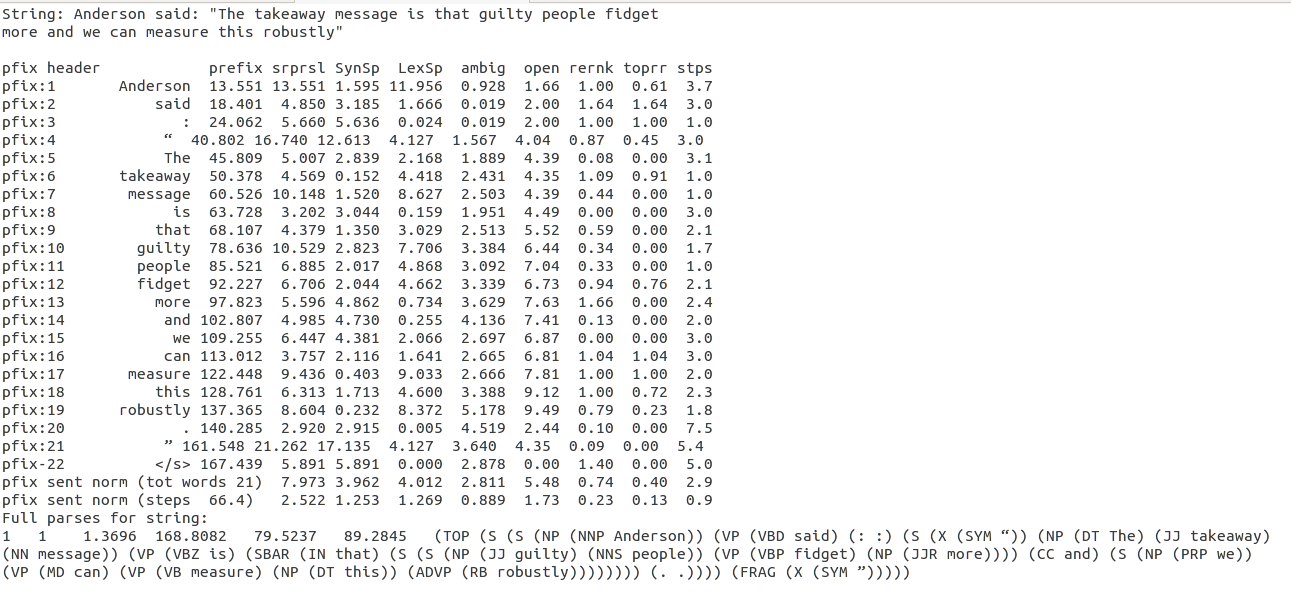
\includegraphics[width=\textwidth]{Roark-Output.png}
\end{frame}

\begin{frame}
\frametitle{Other Parsing Methods}
\framesubtitle{based on different grammar formalisms}
\begin{itemize}
\item Head-driven Phrase Structure Grammar parser
\item Constraint Grammar, Construction Grammar based parsers
\item Link Grammar parser
\item Tree Adjoining Grammar parser
\item Combinatory categorial grammar parser etc.
\end{itemize}
\end{frame}

\begin{frame}
\frametitle{Parsing: Conclusion}
Useful Resources:
\begin{itemize}
\item Theory: Chapters on parsing in J\&M.
\item Vague practice examples: NLTK Chapter 8 (and 7)
\item NLTK code documentation and examples there (not textbook!) 
\item Explore other parsers in Python beyond NLTK
\item Radev's or others' video lectures on parsing
\end{itemize}
\end{frame}

\begin{frame}
\frametitle{}
\Large NLTK Practice Exercises
\end{frame}

\begin{frame}
\frametitle{Exercise-1}
Do Section 1 --3 described in: \\
\url{http://coling.epfl.ch/TP/Parsing.html}
\end{frame}

\begin{frame}
\frametitle{Exercise-2}
How to use Stanford parser and Malt parser in Python with or without NLTK.
\begin{enumerate}
\item My notes on using Stanford parser (stanfordparser.py on BB, in ClassroomMaterials/ProgramSnippets)
\item Useful Links:
\begin{itemize}
\iten \url{http://www.nltk.org/_modules/nltk/parse/stanford.html}
\item \url{http://www.nltk.org/_modules/nltk/parse/malt.html}
\end{itemize}
\end{enumerate}
Note: Once you overcome installation issues, look at the example code I gave, and the links above and sart figuring out what sort of outputs can you get with the parser(s) and where they can be useful for you. 
\end{frame}

\begin{frame}
\frametitle{Next Week}
\begin{enumerate}
\item Topics: 
\begin{itemize}
\item Overview of Semantics and Discourse modeling in NLP
\item Optional theoretical readings: Chapters 19--21 in J\&M
\item Practical Readings: Chapter 2 Section 5, Chapter 10 in NLTK (Chapter 10 is very theoretical according to me).
\item Lectures: 3.1-3.4 in Radev's course (Week 3). 12.1-12.2 in Week 12.
\end{itemize}
\end{enumerate}
\end{frame}
\end{document}

%Tuesday next week: Semantics
%Thursday: Discourse

%\item Overview of NLP applications: Machine Translation, Topic Modeling, Question Answering etc. 
%One way: take task yb task: wsd, ner, srl, discourse analysis etc - get examples of code-software to talk about.
%MT: Talk about Moses and Apertium
%LG: NLG

\begin{frame}
\frametitle{Programming exercise - 1}
\begin{itemize}
\item Take any .txt version file from gutenberg.org, written by your favorite author (in English!)
\item Read that file into your python code, and do the following using NLTK:
\begin{enumerate}
\item Split the file into sentences.
\item Print the following: number of sentences in the file, average sentence length (in number of words), average word length (in number of characters), number of unique words, number of unique stems.
\item Note 1: Once sentence splitting is done, you can ignore punctuation markers for the rest of the calculation.
\item Note 2: You can use any stemmer you want.
\end{enumerate}
\end{itemize}
\end{frame}

\begin{frame}
\frametitle{Programming exercise - 1}
\begin{itemize}
\item For the same file from last slide, do the following:
\item Read that file into your python code, and do the following using NLTK:
\begin{enumerate}
\item Split the file into sentences.
\item For each sentence, print its POS tagged version as a string of tags. E.g., if you have "It is a sentence" as your sentence, and your NLTK tagger outputs the tags for this sentence as a list (or tuple or whatever), you should print the tag as a string. E.g., PRP VBZ DT NN (not as [PRP, VBZ, DT, NN] or as [(It, PRP), (is, VBZ) .. ... ])
\end{enumerate}
\end{itemize}
\end{frame}
